\section{Strategy}
To recognize a facial expression first is needed to find a face in an image, in the online demo it is achieved through Viola Jones while on training and test sets face recognition is automatically done by \textit{Dlib}'s landmark detection.
To extract features at first I considered using LBP histograms but since I was interested only in facial expressions seemed reasonable to use landmark points. 
The key idea is that assuming that similiar expressions have a similiar position on different faces then through an SVM classifier it could be possible to predict someone's "emotion" \footnote{As said earlier someone's emotions are more deep than just their facial expression.}.
In figure \ref{fig:landmarks} is displayed how landmark points are disposed in the used landmark pretrained model, for our purposes were not considered all points but only those defining eyes and the mouth (i.e. points from 37 to 68).
Still is possible for the user to define an arbitrary list of points.
I'm aware that this approach is not the state of the art and to get good results is reccomended to use neural networks ~\cite{blog:emotion}, anyway I was interested in using SVM classifiers and how they would perform.

\begin{figure}[h!t]
    \centering
    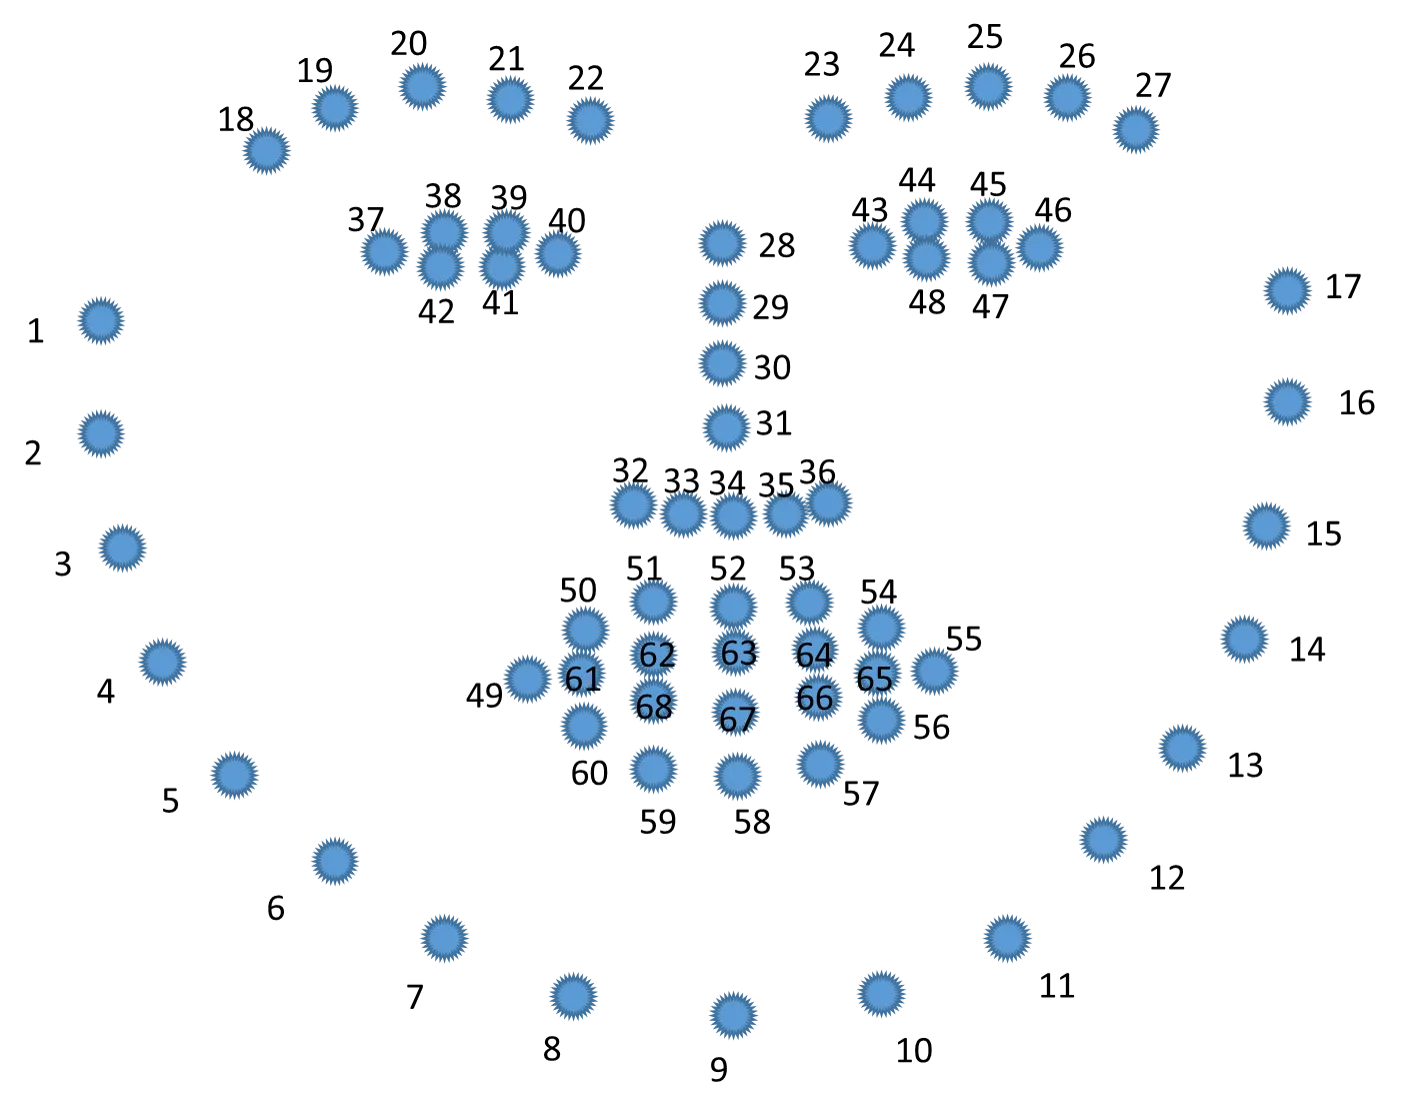
\includegraphics[scale=0.2]{images/landmark.png}
    \caption{Face landmark points from ~\cite{landmark:guide}.}
    \label{fig:landmarks}
\end{figure}

The adopted dataset is the \textit{First Affect-in-the-Wild} (affwild) ~\cite{dataset:affwild}, it consists of 298 videos of which 252 for training and 46 for testing.
I ignored videos in the train set since there are no responses associated to them, these responses are associated to each frame in which a face was identified.
In the dataset are stored relative bounding boxes too but since I was interested in landmark points and the detection is done by \textit{Dlib} I just discarded them.

Emotions are defined as a points on a two dimensional cartesian plane where the abscissa is the \textit{valence}, it expresses if an emotion is positive or negative, and the ordinate is the \textit{arousal}, it discriminates animated emotions from languid ones.
An example of this plane can be seen in figure \ref{fig:emotion_classification}, where are defined 4 different emotions but is possible to have more.
To avoid possible performance reduction I decided to not discriminate between too many classes, and considering also that SVMs in their purest form are binary classifiers it came natural to me to just consider only one response.
I chose valence since it may be more interesting to distinguish between positive and negative expressions rather than exciting or not.

\begin{figure}[h!t]
    \centering
    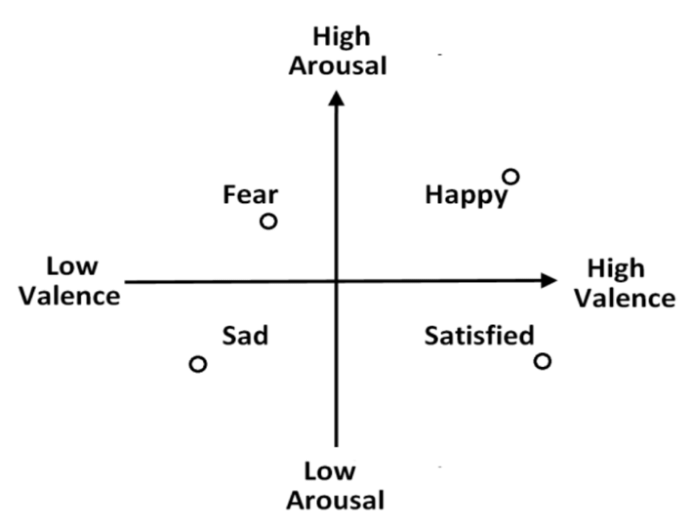
\includegraphics[scale=0.45]{images/emotion-classification.png}
    \caption{Emotion classification model from ~\cite{emotion_classification}.}
    \label{fig:emotion_classification}
\end{figure}
